


\section{Relevant text detection}
\label{cp4:corpus-relevant-text}






Next, \red{we need to determine which 
of the text in the gathered artifacts could} provide information that assists a developer in solving her task.
In our corpus, this text represents \textit{golden data} that one can use to design and evaluate automatic tools that assist developers in the identification of information useful to their tasks. 
To produce it, we 
ask human experts to
mark the text that they deem useful and that provide information for tasks assigned to them~\cite{nadi2020, Robillard2015, marques2020}.



\subsection{Annotation process}


Our intention is that golden data reflect text that instructs developers to perform important actions to accomplish their task~\cite{Robillard2015, Lotufo2012}.
To this end, we describe the text inspected by the annotators, the annotators' background as well as annotation procedures.
% FIXME: find a way to format the standard deviation acronym
\textcolor{white}{\acs{stdv}} % force acronym to appear in the glossary for the time being



\subsubsection{Text inspected}




We restrict the manual identification of text relevant to a task to a random subset of 
50  out of the 300  tasks initially gathered (Section~\ref{cp4:corpus-tasks}).
\gm{-Why select 300? Just select 25 and 25 originally.}
This decision was motivated by the fact that 
creating golden data for the entirety of our tasks 
would require asking human annotators to inspect thousands of artifacts and more than 260,000 sentences, which would be a costly and time-consuming activity. 


% For each one of the 25 Stack Overflow tasks and the 25 GitHub tasks in this subset, we randomly selected 5 artifacts of at least three different types: 
% one API document, a GitHub issue discussion, one Stack Overflow answer, aand two miscellaneous Web pages.
% In total, our corpus contains
% 12,401 unique sentences, with an average of 63.59 sentences per artifact (stdv 66.28).



Although the sentences in the tasks selected for inspection represent
a fraction of the initial number of sentences gathered, 
the number of sentences inspected in \acs{DS-android}
is still significantly higher than 
artifact-specific corpora, such as the \textit{McGill} corpus on information correspondence with 2,445 sentences~\cite{arya2020} or the information types corpus with 4,656 labeled sentences~\cite{Arya2019}.
\art{I'm trying to justify that the size of the corpus is still considerable.}



\begin{table}[!h]
\centering    
\begin{small}
\begin{threeparttable}
\begin{tabular}{lccc}





& \multicolumn{3}{c}{\textbf{\# of sentences}}
\\ \cmidrule(l){2-4} 
& total & mean & stdv  \\

\hline
\hline

\textbf{API documentation} 
& 4,915 & 109.22 & 96.77
\\
\textbf{GitHub issues} 
& 1,890 &  43.95 & 33.69
\\
\textbf{SO answers} 
& 1,420 & 28.40 & 28.48 
\\
\textbf{Miscellaneous Web pages} 
& 4,176 & 70.78 & 56.64 
\\

\hline
\hline
\textbf{Overall} 
& 12,401 & 62.95 & 66.25 
\\
\hline

\end{tabular}
\end{threeparttable}
\end{small}
\caption{Summary statistics for the \acs{DS-android} corpus}
\label{tbl:corpus-summary}
\end{table}




\subsubsection{Annotators}


We recruited 3 graduate students with professional programming experience to produce \textit{golden} data for our corpus. Annotators had to have experience with Java development and they also had to be familiar with the types of artifacts they would encounter throughout the annotation process. 
On average, annotators self-reported 4.6 years of professional
programming experience (stdv 2.49, ranging from 1 to 7 years).



\subsubsection{Annotation procedures}



We divided tasks into batches of 10 tasks each as to avoid fatigue effects~\cite{Ponzanelli2017}. For each batch, annotators had task descriptions and links to artifacts pertinent to the respective task at their disposal. We asked annotators to write a short plan (250 words max~\cite{Rastkar2010}) with instructions that a developer could follow to complete the task successfully. 
The purpose of the plan was to ensure that annotators built enough context about the task.
While perusing artifacts, annotators also had to manually highlight sentences that they deemed useful and that provided information that assisted task completion---instructions similar to the ones used for the creation of the data in the \acs{DS-synthetic} corpus~\cite{marques2020}.


The annotation process was facilitated by a tool we created for this purpose. Figure~\ref{fig:corpus-annotation-tool} shows a screenshot from the tool in 
action, which works as a browser plug-in. The top-right corner panel in the figure shows the browser extension. \red{When an annotator clicked the \texttt{highlight} button, }
the tool instrumented the HTML of a page identifying individual sentences. The tool then allowed annotators to hover over identified sentences and to select them as relevant by clicking on the hovered text. For example, in the first paragraph, an annotator selected  the sentence
``\textit{Call {\small \texttt{ActivityOptions.setLockTaskEnabled()}} ... when starting the activity}'' as relevant to the Android lock mode task (Figure~\ref{fig:lock-screen-task}).







\begin{figure}
    \centering
    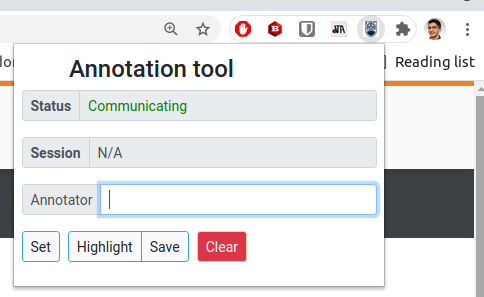
\includegraphics[width=\textwidth]{cp4/annotation-tool}
    \caption{Annotation tool and relevant sentences marked by an annotator}
    \label{fig:corpus-annotation-tool}
\end{figure}




\subsection{Results}


Annotation required a total of \red{$\approx60$} hours of manual work and it was done throughout the course of 4 weeks.
Table~\ref{tbl:corpus-annotation-summary} provides summary statistics for the text marked by 
the annotators over all the artifacts inspected as well as on an artifact type basis.
On average the text deemed useful to a software task in the artifacts inspected comprises 
\red{5} sentences. 
We observe that the highest number of sentences marked originate from \red{artifact type}
while the lowest from \red{artifact} type. Potential explanation for that...


\begin{table}[H]
\centering    
\caption{Summary statistics for the text deemed useful by annotators across the artifacts inspected in the \acs{DS-android} corpus}
\label{tbl:corpus-annotation-summary}
\begin{scriptsize}
\begin{threeparttable}
\begin{tabular}{lcccccc}





& \multicolumn{3}{c}{\textbf{\# of sentences marked}}
& \multicolumn{3}{c}{\textbf{\% of sentences marked by}}
\\ \cmidrule(l){2-4} \cmidrule(l){5-7} 
& total & mean & stdv 
& 1 annot. & 2 annot. & 3 annot. \\

\hline

\textbf{API documentation} 
& 327 & 9.62 & 7.88
& 76\% & 16\% & 7\%
\\
\textbf{GitHub issues} 
& 146 & 4.87 & 3.37
& 74\% & 20\% & 6\%
\\
\textbf{SO answers} 
& 330 & 7.33 & 5.08
& 57\% & 22\% & 21\%
\\
\textbf{Miscellaneous Web pages} 
& 590 & 12.55 & 9.88
& 75\% & 17\% & 8\%
\\

\hline
\textbf{Overall} 
& 1393 & 8.93 & 7.78
& 71\% & 19\% & 10\%
\\
\hline

\end{tabular}
\begin{tablenotes}
    \item[annot] annotator(s);
\end{tablenotes}
\end{threeparttable}
\end{scriptsize}
\end{table}










Since individuals might use different criteria to
assess the usefulness of a sentence to a given task~\cite{Barry1994, Barry1998, Freund2015},
we also report how many sentences marked by the annotators overlap.
Out of \red{n}
unique marked
sentences, 
\red{x} were marked by all annotators,
\red{y} by two of them and the remainder
---\red{z} sentences---by a single annotator.
This result is not surprising and it corroborates 
results on the construction of the \acs{DS-synthetic} 
corpus, where we observe that complete agreement 
occurred on 17\% of the annotated text.
\art{I can also present this data in a bar graph}


\gm{I think a different place is better. The important point here is what
is in the corpus - all sentences marked by annotators and who marked which?}

\clearpage

\begin{landscape}
\begin{table}
\begin{scriptsize}
% \vspace{-3mm}        
\begin{tabular}{cl}
\multicolumn{2}{l}{\cellcolor{lightgray}
    \textbf{Task}
}
\\
\multicolumn{2}{l}{\hspace{3mm}
\parbox[l][0.7cm][c]{16cm}{
    \texttt{No lock screen controls ever
}}}
\href{https://github.com/AntennaPod/AntennaPod/issues/3578}{link}
\\
\multicolumn{2}{l}{\cellcolor{lightgray}
    \textbf{Description}
}
\\
\multicolumn{2}{l}{
\hspace{3mm}
\parbox[l][2.5cm][c]{21cm}{
{\ttfamily
    \ldots
    \\
    \textbf{Expected behaviour:} Lock screen controls
    \\
    \textbf{Current behaviour:} No lock screen controls ever on this phone and never seen them working (or on preceding Huawei P8). Notification controls always work, never had problems. Lock screen controls fine for all other apps without tweaking, same on old P8. I have loosened all notification and lock screen limits, removed power management, etc., but no luck ever. I've also tried setting to use different players, but change in behaviour. \ldots
}}}
% --------------------------------------------------------------------------------------------------
\\
\hline
\hline
\multicolumn{2}{l}{\cellcolor{lightgray}
    \textbf{Artifact}$_1$ - \textbf{API documentation}}
\\
\multicolumn{2}{l}{\hspace{3mm}
\parbox[l][0.7cm][c]{16cm}{
    \texttt{Lock task mode Android Developers
}}}
\href{https://developer.android.com/work/dpc/dedicated-devices/lock-task-mode}{link}
\\
\multicolumn{2}{l}{\cellcolor{lightgray}
    \textbf{Content}}
\\
\texttt{none} & 
\parbox[l][0.6cm][c]{20cm}{
{\ttfamily    
    Android can run tasks in an immersive, kiosk-like fashion called lock task mode.
}}
\\
\texttt{A1} & 
\parbox[l][0.6cm][c]{20cm}{
{\ttfamily    
    Only apps that have been allowlisted by a device policy controller (DPC) can run when the system is in lock task mode.
}} 
\\
\texttt{none} & 
\parbox[l][0.6cm][c]{20cm}{
{\ttfamily    
    A DPC must allowlist apps before they can be used in lock task mode. 
}} 
\\
\texttt{A1, A2} & 
\parbox[l][0.6cm][c]{20cm}{
{\ttfamily    
    Call DevicePolicyManager.setLockTaskPackages() to allowlist apps for lock task mode as shown in the following sample
}} 
\\
\multicolumn{2}{c}{\texttt{...}}
% --------------------------------------------------------------------------------------------------
\\
\hline
\hline
\multicolumn{2}{l}{\cellcolor{lightgray}
    \textbf{Artifact}$_2$ - \textbf{Stack Overflow answer}}
\\
\multicolumn{2}{l}{\hspace{3mm}
\parbox[l][0.7cm][c]{16cm}{
    \texttt{Media Control on Lock Screen like Google Play Music in android?
}}}
\href{https://stackoverflow.com/questions/24652078/media-control-on-lock-screen-like-google-play-music-in-android}{link}
\\
\multicolumn{2}{l}{\cellcolor{lightgray}
    \textbf{Content}}
\\
\texttt{A1, A2, A3} & 
\parbox[l][0.6cm][c]{20cm}{
{\ttfamily    
Have you checked RemoteControlClient? 
}}
\\
\texttt{A2, A3} & 
\parbox[l][0.6cm][c]{20cm}{
{\ttfamily    
    it is used for the Android Music Remote control even if the App is in Lock mode.
}} 
\\
\multicolumn{2}{c}{\texttt{...}}
\\
\hline

\end{tabular}
\end{scriptsize}
\caption{Example of how data is structured in the \acs{DS-android} corpus. Each task has a  title, link, description, and a set of pertinent artifacts. Each artifact has a title, link, and content. For each of the sentences in the content, we store the set of annotators (i.e., \texttt{none}, \texttt{A1}, \texttt{A2}, or \texttt{A3}) who marked the sentence as useful to the task \red{UPDATE after annotation finishes}}
\label{tbl:corpus-data-structure}
\end{table}

\end{landscape}


\clearpage




